%%%%%%%%%%%%%%%%%%%%%%%%%%%%%%%%%%%%%%%%%
% fphw Assignment
% LaTeX Template
% Version 1.0 (27/04/2019)
%
% This template originates from:
% https://www.LaTeXTemplates.com
%
% Authors:
% Class by Felipe Portales-Oliva (f.portales.oliva@gmail.com) with template 
% content and modifications by Vel (vel@LaTeXTemplates.com)
%
% Template (this file) License:
% CC BY-NC-SA 3.0 (http://creativecommons.org/licenses/by-nc-sa/3.0/)
%
%%%%%%%%%%%%%%%%%%%%%%%%%%%%%%%%%%%%%%%%%

%----------------------------------------------------------------------------------------
%	PACKAGES AND OTHER DOCUMENT CONFIGURATIONS
%----------------------------------------------------------------------------------------

\documentclass[
	12pt, % Default font size, values between 10pt-12pt are allowed
	%letterpaper, % Uncomment for US letter paper size
	%spanish, % Uncomment for Spanish
]{fphw}

% Template-specific packages
\usepackage[utf8]{inputenc} % Required for inputting international characters
\usepackage[T1]{fontenc} % Output font encoding for international characters
\usepackage{mathpazo} % Use the Palatino font

\usepackage{graphicx} % Required for including images

\usepackage{booktabs} % Required for better horizontal rules in tables

\usepackage{listings} % Required for insertion of code

\usepackage{enumerate} % To modify the enumerate environment

\usepackage{xcolor}

\definecolor{mGreen}{rgb}{0,0.6,0}
\definecolor{mGray}{rgb}{0.5,0.5,0.5}
\definecolor{mPurple}{rgb}{0.58,0,0.82}
\definecolor{backgroundColour}{rgb}{0.95,0.95,0.92}

\lstdefinestyle{CStyle}{
    backgroundcolor=\color{backgroundColour},   
    commentstyle=\color{mGreen},
    keywordstyle=\color{magenta},
    numberstyle=\tiny\color{mGray},
    stringstyle=\color{mPurple},
    basicstyle=\footnotesize,
    breakatwhitespace=false,         
    breaklines=true,                 
    captionpos=b,                    
    keepspaces=true,                 
    numbers=left,                    
    numbersep=5pt,                  
    showspaces=false,                
    showstringspaces=false,
    showtabs=false,                  
    tabsize=2,
    language=C
}
%----------------------------------------------------------------------------------------
%	ASSIGNMENT INFORMATION
%----------------------------------------------------------------------------------------

\title{OS 2022 Problem Sheet \#2} % Assignment title

\author{Joshua Law} % Student name

\date{September 22th, 2022} % Due date

\institute{Jacobs University Bremen \\ Bachelor Of Computer Science} % Institute or school name

\class{CO-562 Operating Systems} % Course or class name

\professor{Dr. Jurgen Schonwalder} % Professor or teacher in charge of the assignment

%----------------------------------------------------------------------------------------

\begin{document}

\maketitle % Output the assignment title, created automatically using the information in the custom commands above

%----------------------------------------------------------------------------------------
%	ASSIGNMENT CONTENT
%----------------------------------------------------------------------------------------

\section*{Problem 2.1: \emph{process creation using fork() }}

\begin{problem}
Consider the following C program. Assume that all system calls succeed at runtime, that no other
processes are created during the execution of the program, and that process identifiers are allocated sequentially.\end{problem}

\begin{lstlisting}[style=CStyle]
#include <stdio.h>
#include <unistd.h>

static int x = 0;

int main(int argc, char *argv[])
{
	pid_t p = getpid();

	x++;
	fork();
	if (! fork()) {
		if (fork()) {
			x++;
		}
		x++;
	}

	printf("p%d: x = %d\n", getpid() - p, x);
	return 0;
}
\end{lstlisting}
Try to solve this question on paper and not by typing the code into your computer. During an exam, you will have to answer questions like this on paper as well.

\begin{enumerate}[(\itshape a\normalfont)]
	\item How many processes does the program create during its execution. Draw the process tree and indicate the value of x on the edges whenever it changes in a process.
	\item What is the output produced by the program?
\end{enumerate}
%------------------------------------------------

\subsection*{Answer}
\begin{center}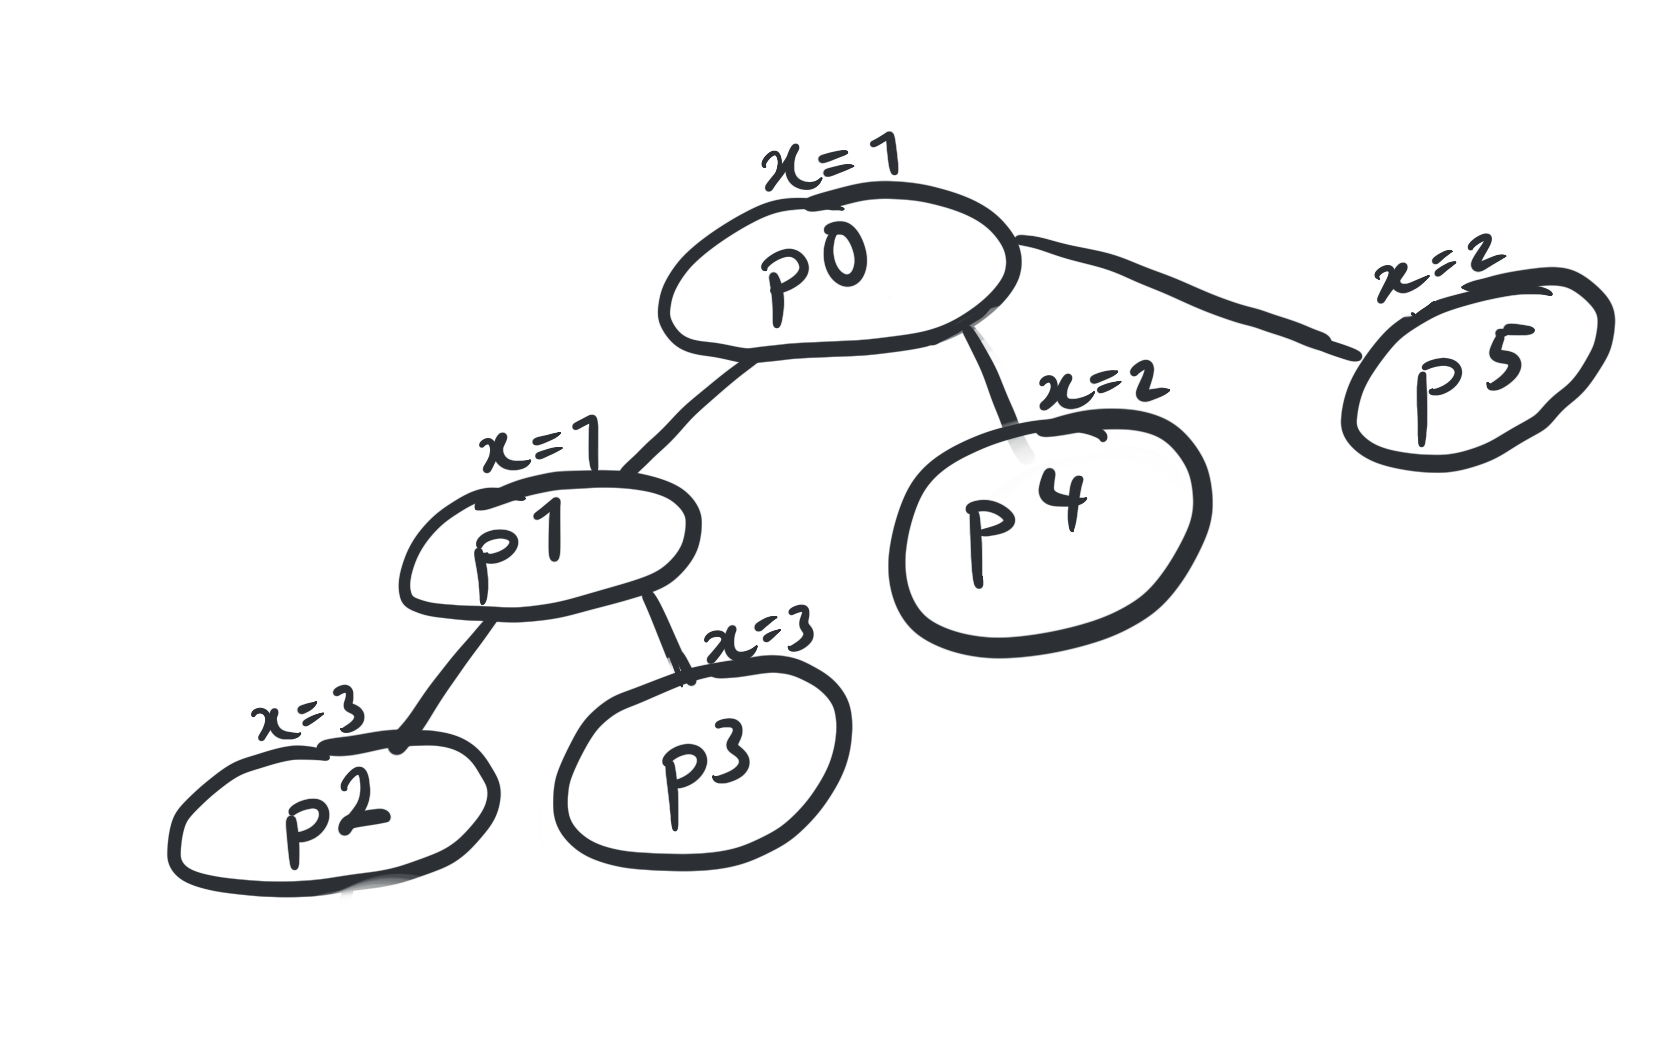
\includegraphics[width=0.7\columnwidth]{process tree.jpg}\end{center}
\begin{enumerate}[(\itshape a\normalfont)]
	\item Total of 6 Processes and the value of X is 7.
	\item p0: x = 1 \newline p1: x = 1 \newline p2: x = 3 \newline p3: x = 3 \newline p4: x = 2 \newline p5: x = 2
\end{enumerate}


%----------------------------------------------------------------------------------------

\section*{Problem 2.2: \emph{xargs - execute a programs with constructed argument lists}}

\begin{problem}
Write a C program called \texttt{xargs}, which is a simplified version of the Unix xargs utility. Your program
reads lines from the standard input and constructs argument lists for a command to be executed. If
more lines are available than can fit on the argument list, then additional commands are executed
with the arguments that did not fit on the first command line. Your program continues constructing
argument lists and executing commands until the end of the standard input has been reached.
The command to execute is specified as part of the xargs arguments or if none are provided, then
\texttt{/bin/echo} is used. Your program should support the following options:
\begin{small}
\begin{description}
	\item \texttt{-n} the (maximum) number of input lines added to the constructed argument lists 
	\item \texttt{-t} show the argument list (on stderr) before the command is executed
\end{description}
\end{small}
If you want to challenge yourself, then you implement the following additional option:
\begin{small}
\begin{description}
	\item \texttt{-j} the (maximum) number of processes (jobs) executed concurrently (default is 1, which means
	processes are executed sequentially)
\end{description}
\end{small}
By implementing this option correctly, you may earn up to two bonus points.
Some examples executions:
\end{problem}
\begin{small}
\begin{lstlisting}[language=bash]
$ echo "hello world" | xargs
hello world
$ seq 0 10 | xargs
0 1 2 3 4 5 6 7 8 9 10
$ seq 0 10 | xargs -t
/bin/echo 0 1 2 3 4 5 6 7 8 9 10
0 1 2 3 4 5 6 7 8 9 10
$ seq 0 10 | xargs -n 3
0 1 2
3 4 5
6 7 8
9 10
$ seq 0 10 | xargs -n 3 -t
/bin/echo 0 1 2
0 1 2
/bin/echo 3 4 5
3 4 5
/bin/echo 6 7 8
6 7 8
/bin/echo 9 10
9 10
$ seq 1 4 | xargs -t -n 1 printf "foo-%02d\n"
printf foo-%02d\n 1
foo-01
printf foo-%02d\n 2
foo-02
printf foo-%02d\n 3
foo-03
printf foo-%02d\n 4
foo-04
\end{lstlisting}
\end{small}
\begin{problem}
Make sure your program properly handles all possible runtime errors and that it returns an error status to its parent process (usually the shell) in case a runtime error occurred.\newline
Your program must use the \texttt{fork()}, \texttt{execvp()}, and \texttt{waitpid()} system calls. Use the \texttt{getopt()}
function of the C library for the command line option parsing. You may want to use the \texttt{getline()}
library function for reading the lines from standard input.
\end{problem}

%------------------------------------------------
\subsection*{Answer}
\begin{lstlisting}[style=CStyle]
#include <stdio.h>
#include <stdlib.h>
#include <unistd.h>
#include <string.h>

int tflag = 0;
int nflag = 0;

int main(int argc, char *argv[])
{
	int opt, arglim = 0;
	char *buffer[128], *buff[64];
	while((opt = getopt(argc,argv,"n:tj:")) != -1){
		switch(opt)
		{
			case 'n':
				arglim = strtol(optarg,NULL,10);
				nflag = 1;
				break;
			case 't':
				tflag = 1;
				break;
			default:
				break;
				return EXIT_FAILURE;
		}
	}
	buff[0] = "/bin/echo";
	if (tflag) {
		int i = 1;
		int len = 0;
		while(getline(&buff[i],&len,stdin) != -1){
			buff[i][strlen(*buff)-1] = '\0';
			fprintf(stderr,"%s",buff[i]);
	}
	}
	if(nflag){
		int c = 0, i = 0;
		while(getline(&buffer[i],0,stdin) != -1)
		{
			int j = getline(&buffer[i],0,stdin);
			c++;
			if(c == arglim){
				pid_t new = fork();
				execvp(buffer[0],buffer);
				if(new == 0){
					waitpid(new,0,0);
				}
				else if(new < 0){
					fprintf(stderr,"Fork error");
				}
				c = 0, i = 0;
			}
			i++;
		}
	} 
	else{
		int i = 1;
		buffer[0] = "/bin/echo ";
		int len = 0;
		buffer[1] = NULL;
		while(getline(&buffer[i],&len,stdin) != -1)
		{
			printf("%s",buffer[0]);
			i++;
		}
		buffer[i] = NULL;
		execvp(buffer[1],buffer);
	}
}
\end{lstlisting}
%----------------------------------------------------------------------------------------


\end{document}
